% !TEX root = ../../main.tex
% !TEX spellcheck = en_US
\section{Evaluation and experimentation methods}
To evaluate our bot we conducted three evaluations and a final experimentation. The first evaluation
was in the design phase of the bot; here we asked StarCraft players on forums\footnote{ Team Liquid:
\url{http://www.teamliquid.net/forum/viewmessage.php?topic\_id=308630}\\ Battle.net:
\url{http://eu.battle.net/sc2/en/forum/topic/3312961916}, accessed 2012-09-03.} what they would like
to see in a teammate bot.  \marginpar{write about features from forum}

Three weeks before the experiment the authors played with BATS to find major bugs to be fixed and
minor improvements that it would benefit from. When the majority of the bugs was fixed, an additional
tester evaluated the bot’s control and behavior to find further improvements before the final experiment.

\paragraph{Player evaluation}
From the player evaluation we conducted that an improvement needed to be made to how commands were
send. For one available commands were not visible to the player, but s/he had to remember them.
This gave the idea to create GUI buttons for the player client. These can be seen in figure
\ref{fig:player_commands_gui}

\begin{figure}[htb]
\centering
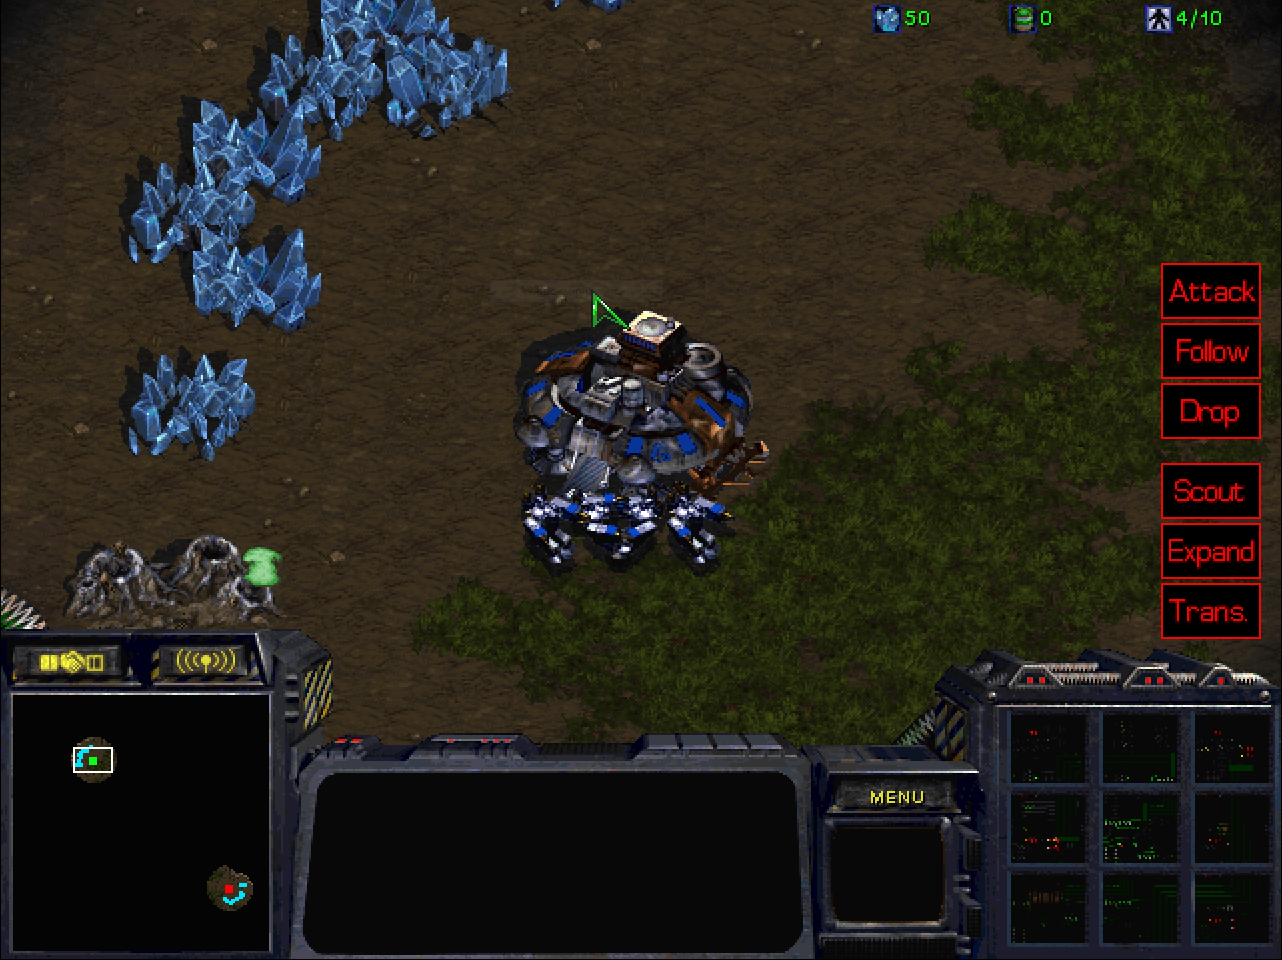
\includegraphics[width=0.8\textwidth]{player_gui_controls}
\caption{Player client with GUI commands enabled}
\label{fig:player_commands_gui}
\end{figure}

\subsection{Experiment method}
The experiment is divided in three parts, first the tester preparation where the testers plays
skirmish matches against the default bot to refresh his/her skills or familiarize him-/herself with
StarCraft and the map the experiment will be conducted on. The testers started the preparation
from a couple of days before the experiment to the day of the experiment.

The second part is the actually experiment itself. Here we present the tester with four scenarios:
\begin{inparaenum}[1\upshape)]
	\item no control over the bot and the bot would not communicate its intentions;
	\item with control over bot, but no communication;
	\item with communication, but no control; and
	\item with both control and communication enabled.
\end{inparaenum}
To avoid a tester preferring a scenario depending on the order they played them all testers played
the scenarios in different orders. This will, however, have a side effect: tester that start with both
communication and control might be overwhelmed with both having a teammate, check its messages, and
be able to control it.

The scenarios are played at fastest game speed, both because normal speed is slow (the experiment
would be too long) and it is considered a standard to play at fastest game speed in the StarCraft
community. Each scenario is limited to 20 minutes—if matches were longer (an hour) the tester might
be bored very quickly and would have to sacrifise a long time of their day. If the tester is winning
after 20 minutes, the tester was asked if we should speed up the game or close it—the matches were
sped up to roughly 10 times faster speed (depending on computer speed), thus the game usually ended
within a minute or two. This was done to let the player win for the experiment to continue to be
interesting.
